\documentclass[11pt,a4paper]{article}

\usepackage[margin=2.5cm]{geometry}
\usepackage{amsmath}
\usepackage{graphicx}
\usepackage{booktabs}
\usepackage{cite}
\usepackage{hyperref}
\usepackage{parskip}
\usepackage{microtype}
\usepackage{caption}
\usepackage{float}
\usepackage{array}
\usepackage{placeins}
\usepackage{needspace}
\usepackage{enumitem}
% A list item is never split across two pages
\setlist[itemize]{itemsep=2pt, topsep=3pt, before={\interlinepenalty=10000\relax}}
\usepackage[T1]{fontenc}
\usepackage{lmodern}
\usepackage[nobottomtitles*]{titlesec}
\usepackage{xcolor}
\usepackage{fancyhdr}
\definecolor{accent}{RGB}{25,60,115}
\titleformat{\section}{\normalfont\Large\bfseries\color{accent}}{\thesection}{0.6em}{}
\titleformat{\subsection}{\normalfont\large\bfseries\color{accent}}{\thesubsection}{0.6em}{}
\pagestyle{fancy}
\fancyhf{}
\fancyhead[L]{\small\color{gray}Assignment 3 · Parallel matrix multiplication}
\fancyhead[R]{\small\color{gray}C.~Falcón Brito}
\fancyfoot[C]{\small\thepage}
\renewcommand{\headrulewidth}{0.4pt}
\setlength{\headheight}{14pt}

% No paragraph leaves a single line at the bottom or at the top of a page
\widowpenalty=10000
\clubpenalty=10000
\displaywidowpenalty=10000
\setlength{\emergencystretch}{1.5em}
\captionsetup{font=small, labelfont={bf,color=accent}, margin=0.5cm}
\renewcommand{\topfraction}{0.9}
\renewcommand{\bottomfraction}{0.8}
\renewcommand{\textfraction}{0.1}
\renewcommand{\floatpagefraction}{0.8}
\renewcommand{\bottomtitlespace}{0.15\textheight}
\titlespacing*{\section}{0pt}{2.6ex plus 0.5ex minus 0.2ex}{1.2ex plus 0.2ex}
\titlespacing*{\subsection}{0pt}{1.8ex plus 0.5ex minus 0.2ex}{0.8ex plus 0.2ex}
\setlength{\intextsep}{14pt plus 4pt minus 2pt}

% Rows of a table generated by analysis/*.py (the primitive input is expandable, so it
% can be followed by \bottomrule inside a tabular)
\makeatletter
\newcommand{\tableinput}[1]{\@@input #1 }
\makeatother

\hypersetup{colorlinks=true, linkcolor=accent, urlcolor=accent, citecolor=accent}

\title{
    \large \textbf{BIG DATA · Academic year 2026-2027} \\[0.4em]
    \LARGE Assignment 3 \\
    \Large Thread Count, Core Sharing and Memory Bandwidth in a Shared-Memory Matrix
    Multiplication with OpenMP \\[0.4em]
    \small Grado en Ciencia e Ingeniería de Datos \\
    \small Universidad de Las Palmas de Gran Canaria
}
\author{Carlos Falcón Brito}
\date{}

\begin{document}

\maketitle
\thispagestyle{empty}

\begin{center}
\textbf{Repository:} \url{https://github.com/Cafabri/Assigment3}
\end{center}

\begin{abstract}
\noindent
This study measures how the number of OpenMP threads changes the time of two C dense
multiplication kernels reused from Assignment~2: a row-wise \texttt{ikj} loop and a
cache-blocked \texttt{ikj}. Each parallel kernel runs the loops of its sequential
counterpart on a contiguous range of rows per thread and is bit-identical to it. Both were
timed on an Intel Core i7-13700KF (8 P-cores with two logical processors each, plus
8 E-cores) for $n = 100$ to $4000$, $p = 1$ to $16$ pinned threads, a scalar and an AVX2
build (median of 15 runs). With one thread per physical core the blocked kernel reached
$S(8) = 7.88$--$7.95$ (efficiency 0.98--1.01) for $n \ge 1000$. Placing a second thread on
each core made it slower ($S(16) = 5.75$--$6.07$), and $p = 12$ was slower still because the
equal row split leaves the threads that share a core behind. The \texttt{ikj} kernel stopped
at $S(8) \approx 5$ once $B$ no longer fit in the L3 cache ($n \ge 2000$), but gained from the
second logical processor ($S(16) \approx 9$). AVX2 multiplied the blocked throughput by
2.7--2.9 at every $p \le 8$, up to 201~GFLOP/s, while its gain on \texttt{ikj} shrank as
threads were added. Parallel execution helped when each core had its own arithmetic units
and the work per call was large; it helped less when threads shared a core or the memory
bandwidth.
\end{abstract}

\section{Introduction and objective}

Assignments~1 and 2 measured sequential kernels. In Assignment~2 the cache-blocked
\texttt{ikj} kernel was the fastest sequential method (1.77~s at $n = 2000$ in the scalar
build, 0.65~s with AVX2), and \texttt{ikj} without blocking was limited by memory reads
once $B$ left the L3 cache. A multicore processor can split the $n^3$ multiply-adds among
cores, but the cores share the L3 cache and the memory bandwidth, the two logical
processors of a core share its execution units, and the cores of this processor are not
all equal. This study asks:

\begin{center}
\begin{minipage}{0.92\textwidth}
\itshape How does the number of threads affect the time, speedup, efficiency and memory of
an OpenMP matrix multiplication compared with its equivalent sequential kernel, and under
which conditions (matrix size, kernel, core sharing, vectorisation) does parallel
execution help?
\end{minipage}
\end{center}

\textbf{Factors varied:} thread count $p$, matrix size $n$, kernel (\texttt{ikj}, blocked),
build (scalar, AVX2) and, in two extensions, the placement of the threads on the logical
processors and the set of processors available (P-cores only, or P- and E-cores).
\textbf{Outcomes:} kernel time, speedup, efficiency and the peak memory of each process.
\textbf{Kept fixed:} language (C), compiler, algorithm and storage layout of each kernel,
float64 values, input matrices, machine.

\textbf{Predictions.} Table~\ref{tab:predictions} lists the predictions. They were committed
to the repository (\texttt{report/hypotheses.md}) while the measurement run was in progress
and before its results were analysed. H5 was formulated after a short smoke test of the
runner ($n \le 250$) showed a drop at $p = 12$, so it is informed by a pilot, not blind.

\begin{table}[H]
\centering
\small
\setlength{\tabcolsep}{4pt}
\begin{tabular}{>{\raggedright\arraybackslash}p{0.7cm}p{14.5cm}}
\toprule
\textbf{Id} & \textbf{Prediction (reason)} \\
\midrule
H1 & Blocked, $n \ge 1000$: $E(p) \ge 0.8$ up to $p = 8$ and $S(16)/S(8) \le 1.2$ (limited by
arithmetic; the two logical processors of a core share its floating-point units) \\
H2 & \texttt{ikj}, $n \ge 2000$: $S(8)$ clearly below 8 and below that of blocked, and
$S(16) > S(8)$ ($B$ no longer fits in the L3 and is streamed from memory for every row of
$C$; a second thread per core can hide part of the memory latency) \\
H3 & $n = 100$: $S(p) < 8$ for every $p$ (fork/join and imbalance of 100 rows are not
negligible against 0.1--0.3~ms of work) \\
H4 & $T(\text{OpenMP}, p = 1) / T_{seq}$ within 2\% of 1 for $n \ge 250$ (same loops; only the
region entry and the row range are added) \\
H5 & (pilot-informed) $E(12) < E(8)$ for both kernels (with 12 threads four cores run two
threads and four run one; equal row ranges make the threads sharing a core finish last) \\
H6 & AVX2/scalar time ratio of blocked about constant in $p$ (2--3$\times$); that of
\texttt{ikj} decreasing with $p$ at $n \ge 2000$ (SIMD does not increase memory bandwidth) \\
H7 & Peak working set $\approx 24n^2$ bytes plus a constant, growing by less than 1~MiB per
thread (the threads share $A$, $B$ and $C$) \\
H8 & All 24 logical processors, threads placed by Windows: $S(24) \le 1.1\,S(16)$, and
$S(32)$, $S(48) < S(24)$ for blocked (slower E-cores with an equal split; time-slicing) \\
\bottomrule
\end{tabular}
\caption{Predictions, evaluated in Section~\ref{sec:hyp} from \texttt{results/report\_numbers.txt}.}
\label{tab:predictions}
\end{table}

\section{Background}

\textbf{Shared-memory parallelism and OpenMP.} OpenMP~\cite{openmp52} expresses
parallelism with compiler directives: a \texttt{parallel} region is executed by a team of
threads (fork) that wait for each other at its end (join). The GNU implementation,
libgomp~\cite{libgomp}, keeps its threads alive between regions, so after the first region a
fork/join costs microseconds, not the creation of threads. The multiplication $C = AB$
parallelises without synchronisation when each thread computes different rows of $C$: $A$
and $B$ are only read, and no element of $C$ is written by two threads.

\textbf{Speedup models.} With $T_{seq}$ the time of the sequential program and $T_p$ that of
the parallel one with $p$ threads, the speedup is $S(p) = T_{seq}/T_p$ and the efficiency
$E(p) = S(p)/p$. If a fraction $f$ of the work is serial, Amdahl's law bounds
$S(p) \le 1 / (f + (1-f)/p)$~\cite{amdahl1967}. The Karp--Flatt metric
$e = (1/S - 1/p) / (1 - 1/p)$ is the value of $f$ that would explain an observed speedup; if
$e$ grows with $p$, the loss comes from overheads that grow with $p$ (imbalance,
contention), not from a fixed serial part~\cite{karpflatt1990}.

\textbf{Resources shared by threads.} A kernel is \textit{compute-bound} when the arithmetic
units limit it and \textit{memory-bound} when the bandwidth or latency of memory does; the
roofline model places a kernel by its operations per byte moved~\cite{williams2009}. The
blocked kernel reuses $b \times b$ tiles from the cache~\cite{lam1991} and is
compute-bound; \texttt{ikj} reads all of $B$ ($8n^2$ bytes) for every row of $C$, which is
cheap while $B$ fits in the cache and limited by memory when it does not. Adding cores adds
arithmetic units and private caches (L1, L2) but not memory bandwidth or L3 capacity.
\textit{Simultaneous multithreading} (SMT, Hyper-Threading) runs two threads on one core:
they share its execution units and L1/L2 caches, which helps when one thread stalls on
memory and can hurt when both need the same units or overflow the shared
cache~\cite{tullsen1995, hennessy2019}.

\textbf{Hybrid processor and vectorisation.} The i7-13700KF combines 8 P-cores (with SMT)
and 8 slower E-cores (without SMT) whose placement Windows decides with hints from the
hardware~\cite{intelopt}; a thread can be restricted to a logical processor with
\texttt{SetThreadAffinityMask}~\cite{setaffinity}. Vectorisation executes one instruction
on 4 doubles (AVX2); gcc vectorises loops whose iterations are independent, here the
innermost $j$ loop of both kernels~\cite{gccopt}.

\textbf{Rounding.} Floating-point addition is not associative~\cite{goldberg1991}. All
kernels add the $n$ products of each $C[i][j]$ in increasing $k$, so splitting rows among
threads does not change any sum and the results are bit-identical.

\section{Methodology}

\subsection{Implementations and reused material}

The sequential baselines are the kernels of Assignment~2
(\url{https://github.com/Cafabri/Assigment2}, commit \texttt{c40444e}, \texttt{c/matmul.c}),
copied unchanged (\texttt{c/matmul.c}, checked with \texttt{diff}): \textbf{\texttt{ikj}}
($j$ innermost, unit-stride rows of $B$ and $C$) and \textbf{blocked} (\texttt{ikj} on
$b \times b$ tiles, tile loops $ii$, $kk$, $jj$). The block sizes are those chosen in
Assignment~2 for each build ($b = 32$ scalar, $b = 256$ AVX2) and were not tuned again. Two
kernels were kept on purpose: one compute-bound and one that becomes memory-bound, so that
the study can show when threads help. The SplitMix64 inputs, the timer and the batching rule
are also those of Assignment~2.

The parallel versions (\texttt{c/parallel.c}) open one \texttt{omp parallel} region with
exactly $p$ threads (\texttt{num\_threads}; \texttt{omp\_set\_dynamic(0)}). Thread $t$
computes the rows $[i_0, i_1)$ of a contiguous split in which the range sizes differ by at
most one row, and runs on them exactly the loops of its sequential kernel (for blocked, the
row tiles start at $i_0$, so a range can end with a shorter tile). The work is divided
statically and equally, and there is no lock, atomic or reduction. All code is my own; no
numerical library is called by any kernel.

\subsection{Input data}

$A$ and $B$ are dense $n \times n$ float64 matrices from the counter-based SplitMix64
generator of Assignment~1 (seed 42 for $A$, 43 for $B$, values uniform in $[0, 10)$,
position $p = i \cdot n + j$), row-major. They are the matrices of Assignments~1 and 2, so
the checksums can be compared across assignments. All values are non-negative, so no
cancellation occurs.

\subsection{Environment}

\textbf{CPU:} Intel Core i7-13700KF; P-cores 0--7 with logical processors $\{0,1\}$,
$\{2,3\}$, \dots, $\{14,15\}$ (read with \texttt{GetLogicalProcessorInformationEx}), E-cores
on logical processors 16--23; 48~KB L1D and 2~MB L2 per P-core, 30~MB shared L3; 31.8~GiB
RAM; Windows 11 Pro, power plan \textit{Balanced}, frequency not fixed. \textbf{Compiler:}
gcc 16.1.0 (MSYS2/MinGW64) with its libgomp; build \texttt{scalar}:
\texttt{-O2 -ffp-contract=off -fopenmp} (the flags of Assignment~2 plus OpenMP); build
\texttt{avx2}: adds \texttt{-fvect-cost-model=dynamic -mavx2}. \textbf{Evidence of
vectorisation:} the gcc report (\texttt{-fopt-info-vec},
\texttt{results/vectorisation\_report.txt}) lists no vectorised kernel loop in the scalar
build and, in the AVX2 build, the innermost $j$ loop of both kernels, sequential and
parallel (\texttt{matmul.c} lines 24 and 43, \texttt{parallel.c} lines 55 and 73), with
32-byte vectors behind a run-time overlap check. \textbf{Analysis:} CPython 3.11.9, NumPy
2.2 (reference results), pandas 2.2, matplotlib 3.10.

\textbf{Thread control.} The runner restricts its process, and so every benchmark process,
to the 16 logical processors of the P-cores. Inside the program, OpenMP thread $t$ pins
itself with \texttt{SetThreadAffinityMask} to entry $t$ of a placement list:
\textbf{spread} $= (0, 2, 4, \dots, 14, 1, 3, \dots, 15)$, one thread per physical core
before any core gets a second one, used in the main experiment; \textbf{compact}
$= (0, 1, 2, \dots, 15)$, two threads per core, used only in an extension. The sequential
kernel runs on the main thread, pinned like thread 0 to logical processor 0. Before timing,
a parallel region checks that the team has exactly $p$ threads; each thread also records the
processor it runs on (\texttt{results/placement.csv}). No numerical library is linked, so no
library creates threads of its own; \texttt{OMP\_PROC\_BIND}, \texttt{OMP\_PLACES} and
\texttt{OMP\_WAIT\_POLICY} are unset (libgomp defaults) and \texttt{OMP\_DYNAMIC=false}.
Oversubscription happens only in the hybrid extension ($p = 32, 48 > 24$ logical
processors).

\subsection{Experiments and measurement protocol}

\textbf{Main experiment (\texttt{threads}).} Both builds, both kernels, the sequential
kernel and its OpenMP version with $p \in \{1, 2, 4, 6, 8, 12, 16\}$, spread placement,
$n \in \{100, 250, 500, 1000, 2000, 4000\}$: 192 configurations. The size sequence was fixed
before running; it ends at $n = 4000$ ($24n^2 = 384$~MB) so that the sequential
\texttt{ikj} (28~s per run) can be repeated 15 times. \textbf{Placement extension:}
compact placement, $p \in \{2, 4, 8, 16\}$, scalar build, $n \in \{1000, 4000\}$.
\textbf{Hybrid extension:} the process may use all 24 logical processors and the threads are
not pinned (Windows places them), $p \in \{1, 8, 16, 24, 32, 48\}$ and the sequential
kernels, scalar build, $n \in \{1000, 4000\}$. This changes two factors at once (available
processors and pinning), so it is compared with the main experiment only qualitatively.

\textbf{Timer.} \texttt{QueryPerformanceCounter} (monotonic) around the kernel call only.
$A$ and $B$ are generated and $C$ allocated and zeroed outside it. For a parallel kernel the
timed call includes entering and leaving the parallel region (fork/join) and the computation
of the row range, but not the creation of the threads, which happens in the untimed check
region. Every unbatched run writes the checksum of $C$, so the computation cannot be
removed.

\textbf{Repetitions.} Each benchmark process makes 2 warm-up runs and 5 measured runs; each
configuration runs in 3 independent processes, interleaved (all configurations once, then
the second and third process of each), so that slow drifts affect all configurations alike:
15 measured runs per configuration. A first call shorter than 10~ms is a separate check
call and the runs are timed in batches of at least 10~ms, reporting the time per call (only
at $n \le 500$; up to 512 calls per batch at $n = 100$). Every raw time is kept
(\texttt{results/raw\_measurements.csv}).

\textbf{Budget.} 15~minutes per run (otherwise the process is killed: TIMEOUT) and 16~GiB of
matrix storage per process (checked before allocating), as in Assignments~1 and 2.

\textbf{Metrics.} $T_{seq}$ and $T_p$ are the \textit{medians} of the 15 measured runs of the
sequential kernel and of its OpenMP version (same build, $n$ and experiment);
$S(p) = T_{seq}/T_p$ and $E(p) = S(p)/p$. The 95\% interval of $S(p)$ is a percentile
bootstrap~\cite{efron1993}: the runs of both configurations are resampled independently
(2000 resamples, fixed seed) and the ratio of medians recomputed. Variability is the IQR of
the 15 runs. Throughput is $2n^3/T$ (GFLOP/s).

\textbf{Memory.} The runner reads the \textit{peak working set} and the \textit{peak private
bytes} of each benchmark process with \texttt{GetProcessMemoryInfo} after it exits; the
\textit{storage} of the matrices is computed, $24n^2$ bytes. These are different quantities
and are reported separately.

\subsection{Correctness}

(1)~At start-up every program checks identity, zero and $2 \times 2$ cases and a
$37 \times 37$ generated input with $b = 5$ (partial tiles, row ranges not multiple of $b$):
both sequential kernels and both parallel kernels with $p \in \{1, 2, 3, 4, 7, 8, 16, 24,
40\}$ (more threads than rows) must equal \texttt{ijk} bit for bit. (2)~For
$n \in \{1, 7, 100, 333, 500\}$, every kernel, build and $p \in \{1, 2, 3, 8, 16, 24\}$
writes its full result, which is compared, on inputs regenerated independently in NumPy,
with an exact NumPy emulation that adds the outer products $A[:,k]\,B[k,:]$ in increasing $k$
(must be bit-identical) and with \texttt{numpy.matmul} (relative tolerance $n u$, with
$u = 2^{-53}$, from the bound $|\hat{C} - C| \le \gamma_n |A||B|$ and $|A||B| = AB$ for
non-negative inputs~\cite{higham2002}). (3)~The checksum of every unbatched run must take a
single value per $n$ across methods, builds, thread counts and placements, and equal the
checksum of Assignment~2 for the same $n$.

\section{Results}

\subsection{Correctness, completeness and variability}

All 708 benchmark processes ended OK (no timeout, memory limit or error; 157~min), so the
largest tested size, $n = 4000$, is the largest attempted, within the budget for every
configuration. All 140 element-wise checks were bit-identical to the exact reference; the
largest difference from \texttt{numpy.matmul} was $3.2 \times 10^{-15}$ (tolerance
$5.6 \times 10^{-14}$ at $n = 500$). For each $n$ a single checksum was observed over 32--54
configurations, equal to that of Assignment~2 at $n = 100$, 1000, 2000 and 4000. Every
pinned thread ran on its requested processor.

Table~\ref{tab:variability} summarises the IQR. For $n \ge 1000$ it is at most 3\% of the
median in 82\% of the configurations; at $n = 4000$ its median is 0.45\%. The short calls
at $n = 100$ (30--250~$\mu$s) vary most (up to 29\%). The sequential \texttt{ikj} at
$n = 1000$ differed by 8\% between processes (medians 0.243--0.262~s), the largest process
spread among the baselines.

\begin{table}[H]
\centering
\small
\begin{tabular}{rccc l}
\toprule
$n$ & Runs & Calls per batch & Median IQR (\% of median) & Largest IQR (\%), configuration \\
\midrule
\tableinput{../results/tables/variability.tex}
\bottomrule
\end{tabular}
\caption{Variability of the 15 measured runs per configuration, main experiment.}
\label{tab:variability}
\end{table}

\subsection{Runtime, speedup and efficiency (scalar build)}

Table~\ref{tab:runtime} gives the medians and Figure~\ref{fig:speedup} the speedup and
efficiency. The sequential times are those of Assignment~2 within a few percent (blocked
1.80~s at $n = 2000$ against 1.77~s there).

\begin{table}[H]
\centering
\small
\setlength{\tabcolsep}{4.5pt}
\begin{tabular}{r r rrrrrrr}
\toprule
& & \multicolumn{7}{c}{OpenMP, $p$ threads (spread placement)} \\
\cmidrule(l){3-9}
$n$ & Sequential & 1 & 2 & 4 & 6 & 8 & 12 & 16 \\
\midrule
\tableinput{../results/tables/runtime_scalar.tex}
\bottomrule
\end{tabular}
\caption{Median time per multiplication, scalar build (15 runs; IQR in
\texttt{results/summary.csv}).}
\label{tab:runtime}
\end{table}

\begin{figure}[H]
\centering
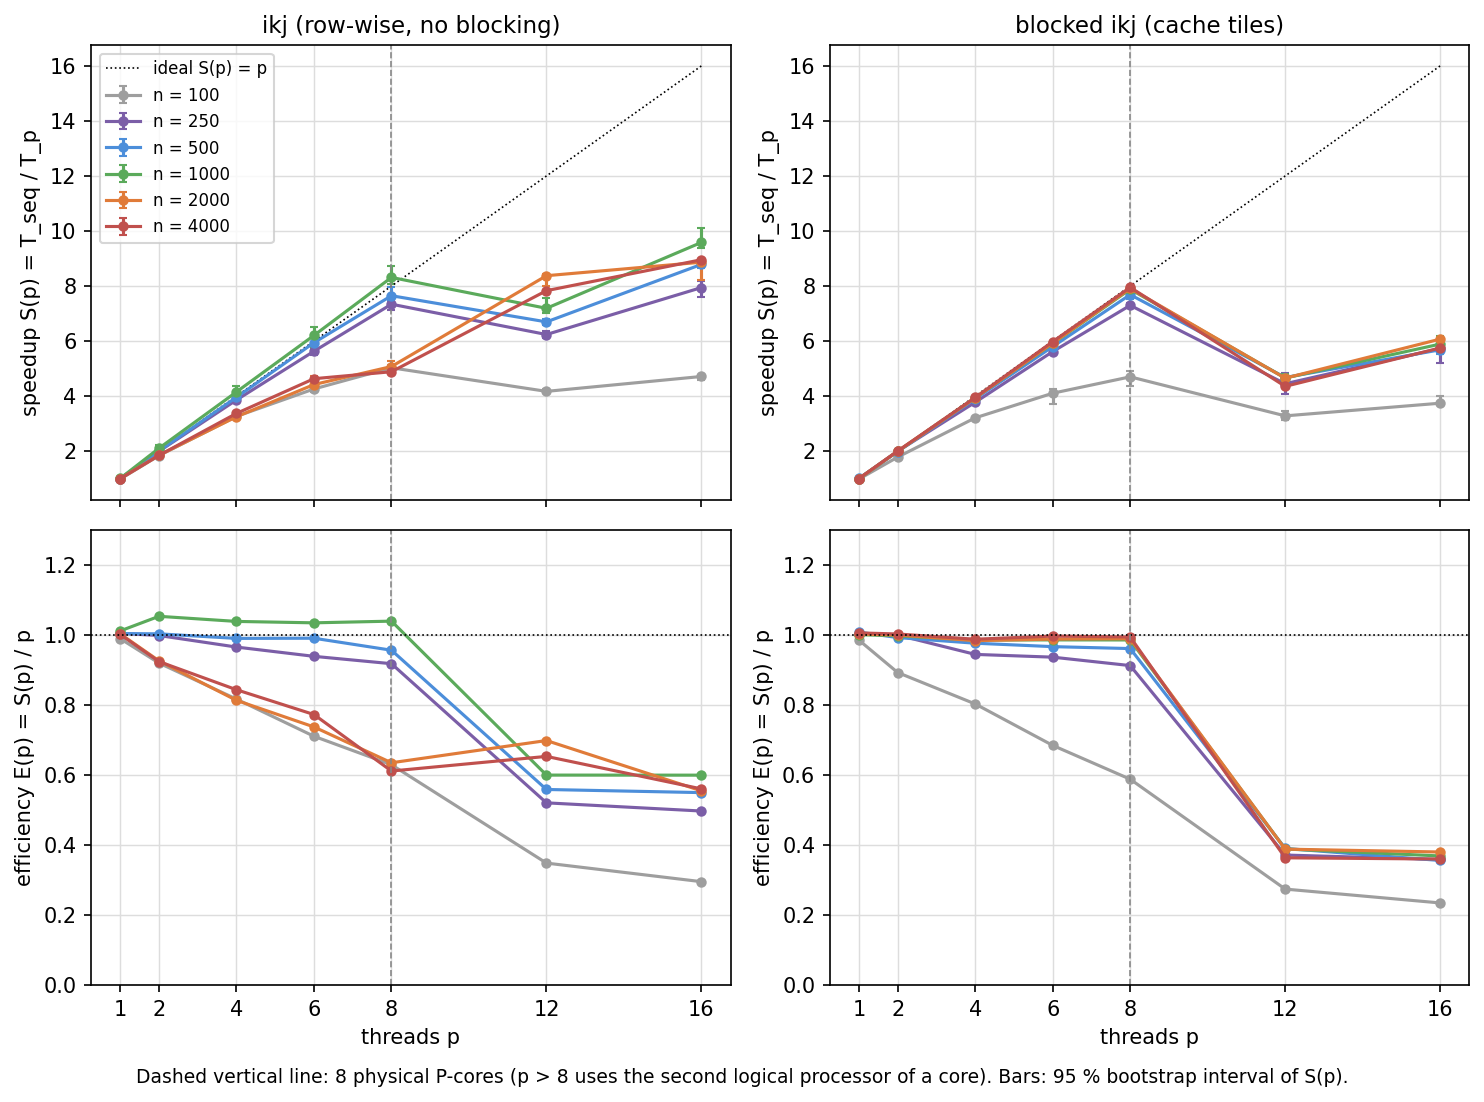
\includegraphics[width=\textwidth]{../results/plot_speedup_scalar.png}
\caption{Speedup (top) and efficiency (bottom) against threads, scalar build, spread
placement. Up to $p = 8$ every thread has its own physical core; beyond, cores get a
second thread. Bars: 95\% bootstrap interval.}
\label{fig:speedup}
\end{figure}

\textbf{Blocked.} For $n \ge 500$ the efficiency stays at 0.96--1.01 up to $p = 8$:
$S(8) = 7.88$, 7.91 and 7.95 at $n = 1000$, 2000 and 4000 (70.5--71.2~GFLOP/s against 8.9
sequential). Beyond $p = 8$ the speedup \textit{drops}: $S(12) = 4.35$--$4.66$ and
$S(16) = 5.75$--$6.07$, so 16 threads are 23--28\% slower than 8.
\textbf{\texttt{ikj}.} At $n \le 1000$ it scales like blocked ($S(8) = 8.31$ at
$n = 1000$). At $n = 2000$ and 4000 the efficiency falls steadily from $p = 2$ and
$S(8) = 5.08$ and 4.89; here the second logical processor helps, $S(16) = 8.87$ and 8.96,
and even $S(12) > S(8)$. \textbf{Small sizes.} At $n = 100$ the speedup peaks at $p = 8$ with
5.03 (\texttt{ikj}) and 4.70 (blocked), 50~$\mu$s per call.

\textbf{One thread.} The OpenMP kernel with $p = 1$ took 0.989--1.015 times the sequential
time for every $n$ and kernel in the scalar build (Figure~\ref{fig:overhead} in the
appendix), i.e.\ the parallel region adds no measurable cost at $n \ge 250$ and about 1.5\%
at $n = 100$ (blocked, 226~$\mu$s).

\textbf{Superlinear points.} Only scalar \texttt{ikj} at $n = 1000$ ($p = 2, 4, 8$;
$S(8) = 8.31$, interval 8.08--8.74), AVX2 \texttt{ikj} at $n = 1000$, $p = 2$ (2.03) and
the AVX2 blocked kernel for $p \le 8$ (Section~\ref{sec:vec}) have a bootstrap interval
entirely above $p$; they are discussed in Section~\ref{sec:super}.

\subsection{Core sharing: placement extension}

Figure~\ref{fig:placement} compares spread and compact placement. With two threads on
\textit{one} core (compact, $p = 2$), blocked ran at 0.83 times the speed of one thread
alone at both sizes, while \texttt{ikj} ran 1.20 ($n = 1000$) and 1.42 ($n = 4000$) times
faster. Compact $p = 8$ (4 cores) gave blocked $S = 2.9$--$3.1$ against 7.9 with spread
(8 cores). With all 16 logical processors both placements use the same processors and
agree within 6\%. For \texttt{ikj} at $n = 4000$ compact $p = 8$ was faster than spread
$p = 8$ (5.41 against 4.89).

\begin{figure}[H]
\centering
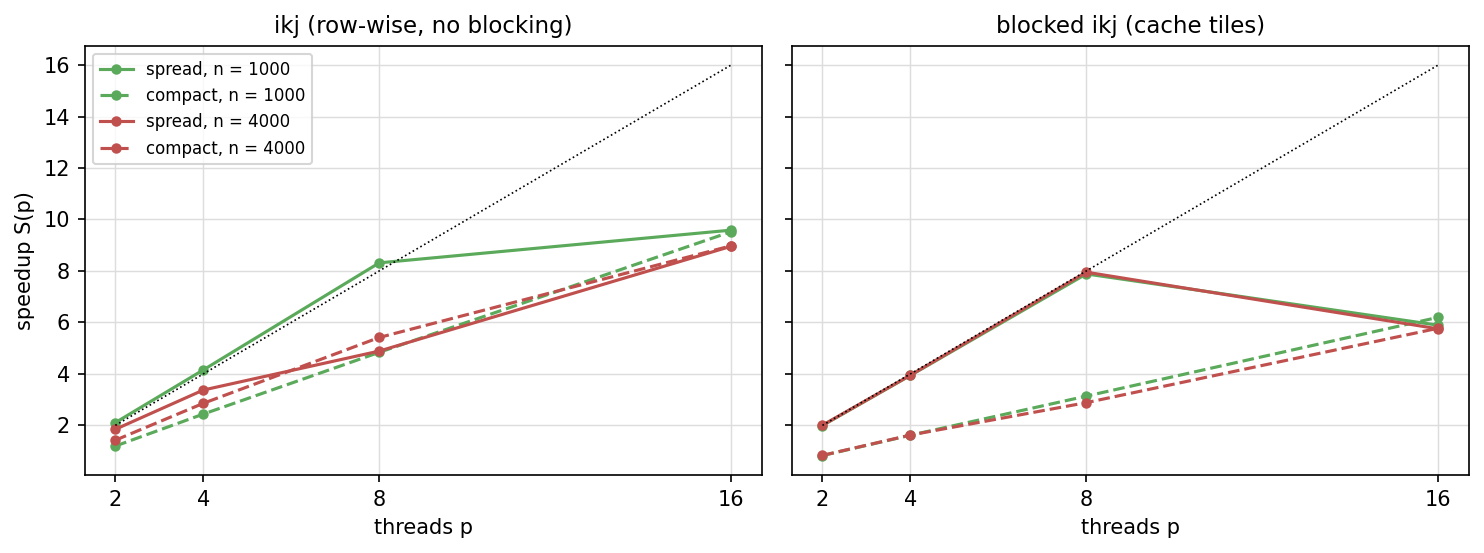
\includegraphics[width=\textwidth]{../results/plot_placement.png}
\caption{Spread (one thread per physical core first) against compact (two threads per
core) placement, scalar build; dotted: $S = p$.}
\label{fig:placement}
\end{figure}

\subsection{Vectorisation extension}
\label{sec:vec}

Figure~\ref{fig:gflops} shows the throughput of both builds and Table~\ref{tab:vec} the
ratio of scalar to AVX2 time at equal kernel, $n$ and $p$, which isolates the SIMD effect
from the thread effect. For blocked the ratio is 2.73--2.86 at every $p \le 8$, so AVX2 and
threads multiply: 189.8--200.8~GFLOP/s at $p = 8$, 21$\times$ the sequential scalar blocked
kernel at $n = 4000$ (14.3~s to 0.674~s). At $p = 12$ and 16 the ratio rises to 3.3--3.5,
because the AVX2 blocked kernel loses less from core sharing ($S(16)/S(8) = 0.92$, against
0.72--0.77 scalar). For \texttt{ikj} at $n = 4000$ the ratio falls from 1.44 (sequential)
to 1.15--1.37 for $p \ge 6$, and at $n = 2000$ from 1.68 to 1.40 at $p = 16$.

\begin{figure}[H]
\centering
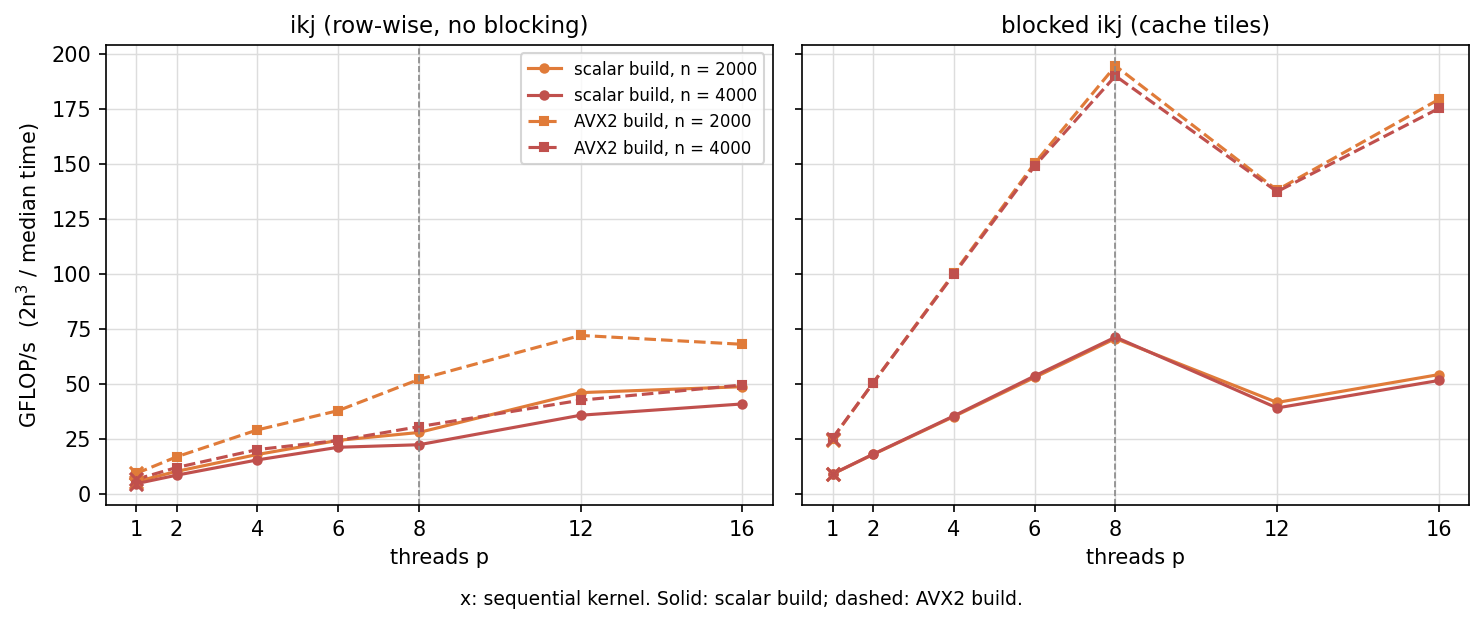
\includegraphics[width=\textwidth]{../results/plot_gflops_builds.png}
\caption{Throughput ($2n^3$ / median time) of the scalar and AVX2 builds at $n = 2000$ and
4000, spread placement.}
\label{fig:gflops}
\end{figure}

\begin{table}[H]
\centering
\small
\setlength{\tabcolsep}{4.5pt}
\begin{tabular}{l r r rrrrrrr}
\toprule
& & & \multicolumn{7}{c}{OpenMP, $p$ threads} \\
\cmidrule(l){4-10}
Kernel & $n$ & Sequential & 1 & 2 & 4 & 6 & 8 & 12 & 16 \\
\midrule
\tableinput{../results/tables/vectorisation.tex}
\bottomrule
\end{tabular}
\caption{$T_{\text{scalar}} / T_{\text{AVX2}}$ (ratio of medians) at the same kernel, $n$
and $p$.}
\label{tab:vec}
\end{table}

In the AVX2 build the OpenMP blocked kernel with one thread was 1.9--2.5\% \textit{faster}
than the sequential one at $n \ge 1000$ ($T_1/T_{seq} = 0.975$--0.981, intervals below 1).
Relative to this one-thread time the speedup is never above $p$ (at most 2.007 at $p = 2$),
so the apparent superlinear speedups of this kernel come from the faster single-thread code
of the parallel version, not from extra parallel gain. At $n = 100$ the AVX2 kernels gain
little from threads ($S \le 2.91$; 87--91~$\mu$s sequential). The AVX2 speedup and runtime
tables are in the appendix.

\subsection{Hybrid extension: E-cores and oversubscription}

With all 24 logical processors available and the placement left to Windows
(Figure~\ref{fig:hybrid}), blocked reached $S(16) = 8.18$--8.52 and $S(24) = 8.83$--9.27
($S(24)/S(16) = 1.08$--1.09) and kept growing slightly when oversubscribed:
$S(48) = 9.04$--9.41. \texttt{ikj} reached $S(24) = 12.52$ at $n = 1000$ (1.29 times
$S(16)$) but not at $n = 4000$ (9.46 against 9.91 at $p = 16$). With 8 threads the
unpinned runs were slower than the pinned spread ones (blocked 5.99--6.78 against
7.88--7.95). A snapshot of the placement found the 8 threads on 7 distinct P-cores and, at
$p = 16$, 14 threads on 7 P-cores and 2 on E-cores; at $p = 48$ all 24 logical processors
were in use. These are single observations of a placement that the scheduler changes
during a run.

\begin{figure}[H]
\centering
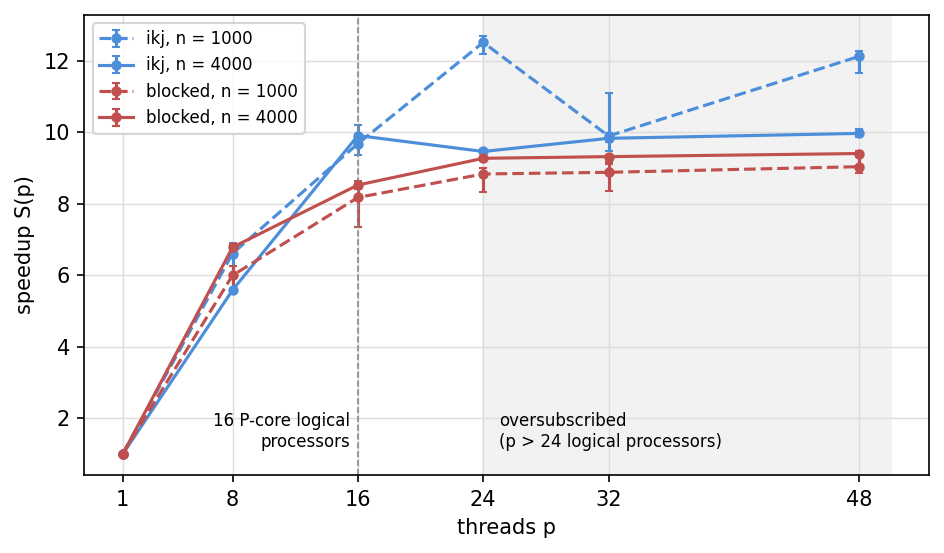
\includegraphics[width=0.72\textwidth]{../results/plot_hybrid.png}
\caption{Hybrid extension: all 24 logical processors, threads placed by Windows, scalar
build; grey: more threads than logical processors.}
\label{fig:hybrid}
\end{figure}

\subsection{Memory}

The peak working set exceeded the $24n^2$ bytes of $A$, $B$ and $C$ by 4.75--5.44~MiB in
every configuration, sequential or parallel, at every $n$ (Table~\ref{tab:memory}): the
threads share the three matrices and the constant part is the program, the C runtime and
libgomp. The peak private bytes grew from $p = 2$ to $p = 16$ by 416--484~KiB at
$n = 4000$, 30--35~KiB per extra thread (stacks and runtime data, mostly reserved rather
than resident). The resolution of these OS counters (pages, and a sampled peak) limits
differences below about 1~MiB.

\begin{table}[H]
\centering
\small
\setlength{\tabcolsep}{4.5pt}
\begin{tabular}{l r r rrrrrrr}
\toprule
& & & \multicolumn{7}{c}{OpenMP, $p$ threads} \\
\cmidrule(l){4-10}
Kernel & $24n^2$ & Sequential & 1 & 2 & 4 & 6 & 8 & 12 & 16 \\
\midrule
\tableinput{../results/tables/memory.tex}
\bottomrule
\end{tabular}
\caption{Peak working set (MiB, median of 3 processes) at $n = 4000$, scalar build, and the
computed storage of $A$, $B$ and $C$.}
\label{tab:memory}
\end{table}

\section{Discussion}

\subsection{Evaluation of the predictions}
\label{sec:hyp}

\begin{table}[H]
\centering
\small
\setlength{\tabcolsep}{4pt}
\begin{tabular}{>{\raggedright\arraybackslash}p{0.7cm}>{\raggedright\arraybackslash}p{3.3cm}p{11cm}}
\toprule
\textbf{Id} & \textbf{Outcome} & \textbf{Evidence} \\
\midrule
H1 & Supported, stronger than predicted & $E(p \le 8) = 0.98$--1.01 (scalar), 0.96--1.03
(AVX2); $S(16)/S(8) = 0.72$--0.77 (scalar) and 0.92 (AVX2): no gain, a loss \\
H2 & Supported & $n \ge 2000$: \texttt{ikj} $S(8) = 4.66$--5.65 against 7.66--7.95 for
blocked; $S(16) = 7.39$--8.96 $> S(8)$ \\
H3 & Supported & $n = 100$: largest $S$ 5.03 (scalar) and 2.91 (AVX2) \\
H4 & Mostly supported & Scalar: 0.989--1.015 at every $n$; AVX2 \texttt{ikj}: within 1\% for
$n \ge 250$; AVX2 blocked: 0.975 at $n = 1000$ (the parallel code is faster), 1.16 at
$n = 100$ \\
H5 & Supported for blocked, not for \texttt{ikj} at $n \ge 2000$ (scalar) & Blocked:
$E(12) = 0.36$--0.48 against $E(8) = 0.96$--1.03. Scalar \texttt{ikj} $n \ge 2000$:
$E(12) = 0.65$--0.70 $> E(8) = 0.61$--0.63 \\
H6 & Supported up to $p = 8$ & Blocked 2.73--2.86 for $p \le 8$ (3.3--3.5 at $p \ge 12$);
\texttt{ikj} $n = 4000$: 1.44 $\to$ 1.15--1.37 \\
H7 & Supported & Peak $-\,24n^2$: 4.75--5.44~MiB for every $p$; $+30$--35~KiB per thread \\
H8 & Partly & Blocked $S(24)/S(16) = 1.08$--1.09, but $S(48) \ge S(24)$; \texttt{ikj}
$n = 1000$: $S(24)/S(16) = 1.29$ \\
\bottomrule
\end{tabular}
\caption{Predictions against the measurements (\texttt{results/report\_numbers.txt}).}
\label{tab:hyp}
\end{table}

\subsection{Why the blocked kernel scales on cores but not on logical processors}

Up to $p = 8$ each thread has its own core, L1 and L2, the tiles of $B$ are reused from
the private caches, and the only shared resource that grows in use (L3 and memory traffic)
stays small for a tiled kernel. The efficiency close to 1 and a Karp--Flatt fraction
$e \le 0.006$ for $p \le 8$ at $n \ge 1000$ show that fork/join and the serial parts are negligible
there. The placement experiment isolates the second logical processor: two threads on one
core gave 0.83 times the throughput of one thread. The core's floating-point units are
already busy with one thread, so a second thread cannot add arithmetic; it only shares the
L1 data cache (48~KB) and the L2. The three $32 \times 32$ tiles of the scalar build occupy
24~KB, so two threads need about all of the L1; the AVX2 build ($b = 256$, tiles in the L2)
lost less ($S(16)/S(8) = 0.92$). This cache explanation is consistent with the two block
sizes but was not measured with hardware counters.

The drop at $p = 12$ follows from the static equal split. Four cores run two threads, four
run one, and every thread gets $n/12$ rows, so the run ends when the slowest threads finish.
If a thread on a shared core progresses at rate $r_2$ (relative to a thread alone) and all
threads at $p = 16$ share cores, then $S(16) \approx 16 r_2$ and $S(12) \approx 12 r_2 =
12\,S(16)/16$. This model, using only the measured $S(16)$, predicts $S(12) = 4.31$--4.55
(scalar) and 5.29--5.67 (AVX2) against measured 4.35--4.66 and 5.53--5.70. A dynamic
schedule or an uneven split would let faster threads take more rows; this was not tested.

\subsection{Why \texttt{ikj} saturates, and when SMT helps}

\texttt{ikj} reads all of $B$ for each row of $C$. At $n = 1000$, $B$ (8~MB) stays in the
30~MB L3 and each core streams it at its own rate, so \texttt{ikj} scales like blocked. At
$n \ge 2000$, $B$ (32--128~MB) no longer fits and is read from memory for every row, and
eight threads reach only 22.3~GFLOP/s at $n = 4000$ (against 71.2 for blocked). The
Karp--Flatt fraction is already 0.06--0.09 from $p = 2$ to 8 (against $e < 0$ at
$n = 1000$). The metric alone cannot separate a serial part from contention, but the
parallel region of this kernel contains only the row loops, and the loss appears exactly
when $B$ leaves the L3, so the likely cause is that the threads compete for the shared
memory bandwidth. Here the second logical processor helps (1.42 times one thread on one core at
$n = 4000$): while one thread waits for memory, the other computes. This is also why compact
$p = 8$ beat spread $p = 8$ for \texttt{ikj} at $n = 4000$: two threads on a core share
its L2 and read the same rows of $B$ at about the same time. The same limit explains H6:
AVX2 shortens the arithmetic but not the wait for memory, so its gain shrinks as threads
saturate the bandwidth. The memory bandwidth itself was not measured.

\subsection{Small sizes, one thread and superlinear points}
\label{sec:super}

At $n = 100$ a call lasts 30--250~$\mu$s. Each of up to 16 threads gets 6--7 rows, and
a fork/join of the pool plus the uneven end of the threads becomes a visible fraction:
$S \le 5.03$ (scalar) and $\le 2.91$ (AVX2, whose sequential call is already 3$\times$
shorter). With one thread the parallel kernel costs the same as the sequential one in the
scalar build. In the AVX2 build the blocked parallel kernel is about 2\% faster; its code
differs only in how the row bounds are passed (\texttt{blocked\_rows} receives
$[i_0, i_1)$), so the compiler may lay out or align the loops differently. This was not
analysed at the instruction level. The superlinear points of scalar \texttt{ikj} at
$n = 1000$ are 1--4\% above $p$, the lower bound of the interval only 1\% above at
$p = 8$, and coincide with the largest process spread of a baseline (8\%). A plausible
cause, shared reads of $B$ in the L3 by threads that progress together, was not measured,
so these points are reported as small and not explained.

\subsection{E-cores and oversubscription}

The hybrid runs had 8 more cores available, so their higher $S(16)$ for blocked (8.2--8.5
against 5.8--6.1 pinned) does not mean that the Windows placement is better; it means that
16 threads spread over P- and E-cores did more than 16 threads on 8 cores, each of which
delivers only 0.83 of its single-thread throughput when shared. With 8 threads the unpinned runs were slower than pinned ones:
the scheduler did not always use 8 distinct cores. Oversubscription did not reduce the
blocked speedup, contrary to H8: with 48 threads each gets fewer rows, and threads that
finish early free a processor for waiting ones, which acts like a dynamic schedule over
fast and slow cores. This interpretation follows from the static row split and was not
tested directly. The \texttt{ikj} results at $n = 1000$ vary strongly with $p$ (9.90 at
$p = 32$, 12.52 at $p = 24$) and have wide intervals; they are reported, not interpreted.

\subsection{Answer to the research question}

For these kernels and this machine, parallel execution helped most when (i) each thread had
its own physical core, (ii) the kernel was limited by arithmetic (blocked, efficiency
0.96--1.03 at $p \le 8$, $n \ge 500$, both builds) and (iii) a call took at least about a
millisecond. It helped less when the threads shared the memory bandwidth (\texttt{ikj},
$n \ge 2000$: $S(8) \approx 5$), and it hurt when two compute-bound threads shared a core,
alone (0.83) or mixed with unshared cores under an equal split ($p = 12$). The second logical
processor of a core paid off only for the memory-bound kernel. Vectorisation was
complementary for the compute-bound kernel (2.7--2.9$\times$ at every $p \le 8$), and its
gain fell as the memory-bound kernel approached the bandwidth limit. The extra memory of the
threads was negligible (about 30~KiB each).

\subsection{Limitations}

One machine, compiler and OS; frequency not fixed (Balanced plan), so turbo frequency may
fall as more cores are active, which lowers $S(p)$ and is included in the measured
speedups. No hardware counters: the cache, bandwidth and SMT explanations are inferred from
timings, block sizes and placement experiments. Block sizes were tuned in Assignment~2 for
one thread, not for each $p$. Only a static equal row split was tested. The hybrid extension
changes the available processors and the pinning at once, and its placement observations
are snapshots. The peak-memory counters cannot resolve per-thread costs below about 1~MiB.
Different machines, compilers or schedules can change all of these numbers.

\section{Conclusions}

Within the tested kernels, sizes ($n \le 4000$), builds and the i7-13700KF:
\begin{itemize}
    \item An OpenMP row split of the blocked kernel is bit-identical to the sequential
    kernel and scales almost ideally on physical cores: $S(8) = 7.9$ for $n \ge 1000$, with
    no measurable cost at $p = 1$.
    \item Putting a second compute-bound thread on a core lowered the throughput of the core
    (0.83), and mixing shared and unshared cores under an equal split made $p = 12$ the
    worst configuration above $p = 8$; a simple imbalance model reproduces it.
    \item The row-wise \texttt{ikj} kernel is limited by memory once $B$ leaves the L3:
    $S(8) \approx 5$, and the second logical processor recovers part of the loss
    ($S(16) \approx 9$).
    \item AVX2 and threads combine for the compute-bound kernel (up to 201~GFLOP/s, 21$\times$
    the scalar sequential kernel), but AVX2 gains less as a memory-bound kernel uses more
    threads.
    \item Threads add negligible memory: the three matrices are shared.
\end{itemize}

\textbf{Open questions.} Hardware-counter evidence for the SMT and bandwidth explanations;
dynamic or uneven scheduling on shared and hybrid cores; block sizes tuned per thread count;
the cause of the small superlinear points of \texttt{ikj} at $n = 1000$; and the
distributed version of Assignment~4, which will reuse these kernels.

\section*{Reproducibility}

The repository holds the code, the exact commands (\texttt{README.md}), the raw data and the
analysis scripts. \texttt{python run\_experiment.py} builds both binaries and runs all
three experiments (157~min here); \texttt{analysis/check\_correctness.py},
\texttt{plot\_results.py} and \texttt{report\_numbers.py} regenerate the validation, the
figures, the tables and every number in this report.

\section*{Use of generative AI}

Claude Opus 5.5 (Anthropic), used through Claude Code, served as a support tool during this
assignment: to help plan the study, write and debug the parallel kernels, the benchmark
program, the experiment runner and the analysis scripts, and to draft and revise the
wording of the report. All the measurements come from running the code on the machine
described in Section~3.3, and every number in the text is produced by
\texttt{analysis/report\_numbers.py} from the raw data. The author reviewed the code and
the AI-generated text, checked the numbers against the raw data and the references, and is
responsible for the conclusions.

{\footnotesize
\begin{thebibliography}{14}
\setlength{\itemsep}{0pt}\setlength{\parsep}{0pt}

\bibitem{openmp52}
OpenMP Architecture Review Board, \textit{OpenMP Application Programming Interface,
Version 5.2}, Nov. 2021. [Online]. Available: \url{https://www.openmp.org/specifications/}

\bibitem{libgomp}
Free Software Foundation, \textit{GNU Offloading and Multi Processing Runtime Library: The
GNU OpenMP and OpenACC Implementation}. [Online]. Available:
\url{https://gcc.gnu.org/onlinedocs/libgomp/}. Accessed: Nov. 12, 2026.

\bibitem{amdahl1967}
G.~M. Amdahl, ``Validity of the single processor approach to achieving large scale
computing capabilities,'' in \textit{Proc. AFIPS Spring Joint Computer Conf.}, 1967,
pp.~483--485, doi: 10.1145/1465482.1465560.

\bibitem{karpflatt1990}
A.~H. Karp and H.~P. Flatt, ``Measuring parallel processor performance,''
\textit{Commun. ACM}, vol.~33, no.~5, pp.~539--543, May 1990, doi: 10.1145/78607.78614.

\bibitem{williams2009}
S.~Williams, A.~Waterman, and D.~Patterson, ``Roofline: An insightful visual performance
model for multicore architectures,'' \textit{Commun. ACM}, vol.~52, no.~4, pp.~65--76,
Apr. 2009, doi: 10.1145/1498765.1498785.

\bibitem{lam1991}
M.~D. Lam, E.~E. Rothberg, and M.~E. Wolf, ``The cache performance and optimizations of
blocked algorithms,'' in \textit{Proc. 4th Int. Conf. Architectural Support for
Programming Languages and Operating Systems (ASPLOS IV)}, 1991, pp.~63--74,
doi: 10.1145/106972.106981.

\bibitem{tullsen1995}
D.~M. Tullsen, S.~J. Eggers, and H.~M. Levy, ``Simultaneous multithreading: Maximizing
on-chip parallelism,'' in \textit{Proc. 22nd Annu. Int. Symp. Computer Architecture
(ISCA)}, 1995, pp.~392--403, doi: 10.1145/223982.224449.

\bibitem{hennessy2019}
J.~L. Hennessy and D.~A. Patterson, \textit{Computer Architecture: A Quantitative
Approach}, 6th~ed. Cambridge, MA, USA: Morgan Kaufmann, 2019.

\bibitem{intelopt}
Intel Corporation, \textit{Intel 64 and IA-32 Architectures Optimization Reference Manual}.
[Online]. Available:
\url{https://www.intel.com/content/www/us/en/developer/articles/technical/intel-sdm.html}.
Accessed: Nov. 12, 2026.

\bibitem{setaffinity}
Microsoft, ``SetThreadAffinityMask function (winbase.h),'' Win32 API documentation.
[Online]. Available:
\url{https://learn.microsoft.com/en-us/windows/win32/api/winbase/nf-winbase-setthreadaffinitymask}.
Accessed: Nov. 12, 2026.

\bibitem{gccopt}
Free Software Foundation, ``Options that control optimization,'' in \textit{Using the GNU
Compiler Collection (GCC)}. [Online]. Available:
\url{https://gcc.gnu.org/onlinedocs/gcc/Optimize-Options.html}. Accessed: Nov. 12, 2026.

\bibitem{goldberg1991}
D.~Goldberg, ``What every computer scientist should know about floating-point
arithmetic,'' \textit{ACM Comput. Surv.}, vol.~23, no.~1, pp.~5--48, Mar. 1991,
doi: 10.1145/103162.103163.

\bibitem{higham2002}
N.~J. Higham, \textit{Accuracy and Stability of Numerical Algorithms}, 2nd~ed.
Philadelphia, PA, USA: SIAM, 2002.

\bibitem{efron1993}
B.~Efron and R.~J. Tibshirani, \textit{An Introduction to the Bootstrap}. New York, NY,
USA: Chapman \& Hall, 1993.

\end{thebibliography}
}

\clearpage
\appendix
\section*{Appendix: AVX2 build and one-thread overhead}

\begin{table}[H]
\centering
\small
\setlength{\tabcolsep}{4.5pt}
\begin{tabular}{r r rrrrrrr}
\toprule
& & \multicolumn{7}{c}{OpenMP, $p$ threads (spread placement)} \\
\cmidrule(l){3-9}
$n$ & Sequential & 1 & 2 & 4 & 6 & 8 & 12 & 16 \\
\midrule
\tableinput{../results/tables/runtime_avx2.tex}
\bottomrule
\end{tabular}
\caption{Median time per multiplication, AVX2 build (15 runs).}
\label{tab:runtime_avx2}
\end{table}

\begin{table}[H]
\centering
\small
\setlength{\tabcolsep}{5pt}
\begin{tabular}{r rrrrrrr}
\toprule
$n$ & $p = 1$ & 2 & 4 & 6 & 8 & 12 & 16 \\
\midrule
\tableinput{../results/tables/speedup_avx2.tex}
\bottomrule
\end{tabular}
\caption{Speedup $S(p)$ and, in small type, efficiency $E(p)$, AVX2 build. The scalar
values are plotted in Figure~\ref{fig:speedup}; all values with bootstrap intervals and the
Karp--Flatt metric are in \texttt{results/speedup.csv}.}
\label{tab:speedup_avx2}
\end{table}

\begin{figure}[H]
\centering
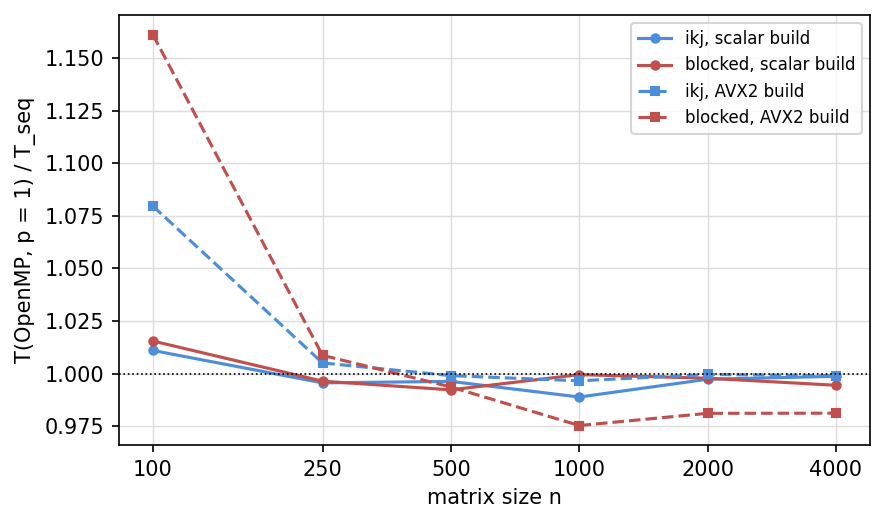
\includegraphics[width=0.62\textwidth]{../results/plot_overhead_p1.png}
\caption{Time of the OpenMP kernel with one thread relative to the sequential kernel.}
\label{fig:overhead}
\end{figure}

\end{document}
